%!Tex Root = ../main.tex
% ./Packete.tex
% ./Design.tex
% ./Deklarationen.tex
% ./Vorbereitung.tex
% ./Aufgabe2.tex
% ./Aufgabe3.tex
% ./Aufgabe4.tex
% ./Bonus.tex

\section{Aufgabe 1}

\setcounter{exercise}{1}

\begin{frame}[fragile, allowframebreaks]{Aufgabe \thesection}{RETI}
    % \begin{requirementsnoinc}
    % \end{requirementsnoinc}
    \begin{exercisenoinc}
      Es gilt für $n\ge 0$:
      \begin{align*}
        &f(0) = 0\\
        &f(1) = 1\\
        &f(n)={f(n-1)+f(n-2)}\qquad (\text{für}\;n\geq2)
      \end{align*}
    \end{exercisenoinc}
    \begin{solutionnoinc}
      \numberedcodebox[minted language=c, minted options={fontsize=\tiny,linenos}]{./figures/example_fib_it_simple.picoc}
    \end{solutionnoinc}
    \begin{solutionnoinc}
      \begin{columns}
        \begin{column}[t]{0.5\textwidth}
          \numberedcodebox[minted language=text, minted options={fontsize=\tiny,linenos}]{./figures/fib_it_simple.reti}
        \end{column}
        \begin{column}[t]{0.5\textwidth}
          \numberedcodebox[minted language=text, minted options={fontsize=\tiny,linenos,firstnumber=13}]{./figures/fib_it_simple_2.reti}
        \end{column}
      \end{columns}
      \vspace{0.5cm}
    \end{solutionnoinc}
    \begin{solutionnoinc}
      \centering
      \href{https://asciinema.org/a/583721}{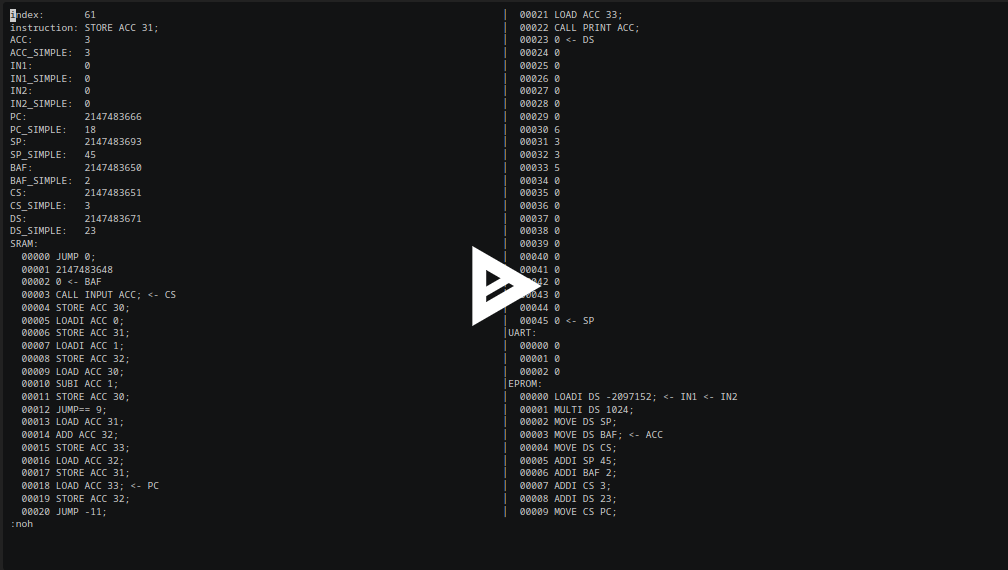
\includegraphics[width=0.6\textwidth]{./figures/fib_video.png}}
    \end{solutionnoinc}
    % highlightlines={5,15,18}
\end{frame}
